% DOKUMENTACE ZÁVĚREČNÉ STUDIJNÍ PRÁCE - MAGE SURVIVOR
%%%%%%%%%%%%%%%%%%%%%%%%%%%%%%%%%%%%%%%%%%%%
\documentclass[12pt, a4paper,
oneside
]{report}

\AtBeginDocument{%
	\immediate\write16{(cleaning stray figureversions output...)}%
	\thispagestyle{empty}
	\let\superiorSup\relax
	\let\textOsF\relax
	\let\textTOsF\relax
	\let\liningLF\relax
	\let\liningTLF\relax
	\let\tabularTab\relax
	\let\proportionalProp\relax
	\let\tabularmath\relax
	\let\proportionalmath\relax
	\let\fontspechyperref\relax
}

%% Proměnné
\newcommand\obor{INFORMAČNÍ TECHNOLOGIE}
\newcommand\kodOboru{18-20-M/01}
\newcommand\zamereni{se zaměřením na počítačové sítě a programování}
\newcommand\skola{Střední škola průmyslová a umělecká, Opava}
\newcommand\trida{IT4}
\newcommand\jmenoAutora{Ondřej Jasník}
\newcommand\skolniRok{2025/26}
\newcommand\datumOdevzdani{31. 12. 2025}
\newcommand\nazevPrace{Mage Survivor: hra vytvořena v Godot Enginu}

\title{\nazevPrace}
\author{\jmenoAutora}
\date{\datumOdevzdani}

\usepackage[top=2.5cm, bottom=2.5cm, left=3.5cm, right=1.5cm]{geometry}

\usepackage[czech]{babel}
\usepackage[utf8]{inputenc}
\usepackage[T1]{fontenc}
\usepackage{cmap}

\usepackage{graphicx}
\usepackage{subcaption}
\usepackage[hidelinks]{hyperref}

\linespread{1.25}
\setlength{\parskip}{0.5em}

\usepackage[pagestyles]{titlesec}
\titleformat{\chapter}[block]{\bfseries\LARGE}{\thechapter}{10pt}{\vspace{0pt}}
\titleformat{\section}[block]{\bfseries\Large}{\thesection}{10pt}{\vspace{0pt}}
\titleformat{\subsection}[block]{\bfseries\large}{\thesubsection}{10pt}{\vspace{0pt}}

\usepackage{tocloft}
\setlength{\cftbeforechapskip}{0pt}
\setlength{\cftbeforesecskip}{0pt}

\setcounter{secnumdepth}{2}
\setcounter{tocdepth}{1}
\usepackage{fancyhdr}
\pagestyle{fancy}
\renewcommand{\headrulewidth}{0.025pt}
\fancyhf{}
\fancyhead[R]{\thepage}
\fancyhead[L]{\nouppercase{\leftmark}}

\usepackage{booktabs}
\usepackage{url}
\usepackage{pdfpages}
\usepackage{upgreek}
\usepackage{amsmath}
\usepackage{amsfonts}

\makeatletter
\@namedef{ver@figureversions.sty}{9999/99/99}
\newcommand{\DeclareFigureVersion}[2]{}
\newcommand{\figureversion}[1]{}
\makeatother

\makeatletter
\providecommand{\superiorSup}{}
\providecommand{\textOsF}{}
\providecommand{\textTOsF}{}
\providecommand{\liningLF}{}
\providecommand{\liningTLF}{}
\providecommand{\tabularTab}{}
\providecommand{\proportionalProp}{}
\providecommand{\tabularmath}{}
\providecommand{\proportionalmath}{}
\makeatother

\usepackage{listings}
\usepackage{xcolor}
\usepackage{float}  % Pro float=H (zde definitvně)

\renewcommand{\lstlistingname}{Kód}
\renewcommand{\lstlistlistingname}{Seznam programových kódů}

% Nastavení barev
\definecolor{mediumgray}{rgb}{0.3, 0.4, 0.4}
\definecolor{mediumblue}{rgb}{0.0, 0.0, 0.8}
\definecolor{forestgreen}{rgb}{0.13, 0.55, 0.13}
\definecolor{darkviolet}{rgb}{0.58, 0.0, 0.83}
\definecolor{royalblue}{rgb}{0.25, 0.41, 0.88}
\definecolor{crimson}{rgb}{0.86, 0.8, 0.24}

% Nastavení pro GDScript (podobné Python)
\lstdefinestyle{GDScript}{
	language=Python,
	backgroundcolor=\color{white},
	basicstyle=\ttfamily\small,
	breakatwhitespace=false,
	breaklines=true,
	captionpos=b,
	columns=fullflexible,
	commentstyle=\color{mediumgray}\upshape,
	emph={},
	emphstyle=\color{crimson},
	extendedchars=true,
	fontadjust=true,
	frame=single,
	identifierstyle=\color{black},
	keepspaces=true,
	keywordstyle=\color{mediumblue},
	keywordstyle={[2]\color{darkviolet}},
	keywordstyle={[3]\color{royalblue}},
	literate=%
	{á}{{\'a}}1 {č}{{\v{c}}}1 {ď}{{\v{d}}}1 {é}{{\'e}}1 {ě}{{\v{e}}}1
	{í}{{\'i}}1 {ň}{{\v{n}}}1 {ó}{{\'o}}1 {ř}{{\v{r}}}1 {š}{{\v{s}}}1
	{ť}{{\v{t}}}1 {ú}{{\'u}}1 {ů}{{\r{u}}}1 {ý}{{\'y}}1 {ž}{{\v{z}}}1,		
	numbers=left,
	numbersep=5pt,
	numberstyle=\tiny\color{black},
	rulecolor=\color{black},
	showlines=true,
	showspaces=false,
	showstringspaces=false,
	showtabs=false,
	stringstyle=\color{forestgreen},
	tabsize=4,
	title=\lstname,
	upquote=true
	% Floatování vypnuto - kód je vložen inline
}

\setlength{\headheight}{15pt}

\begin{document}
	
	\pagestyle{empty}
	\pagenumbering{Roman}
	
	\clearpage

%% Titulní stránka
%%%%%%%%%%%%%%%%%%%%%%%%%%%%%%%%%%%%%%%%
		\begin{figure}[h]
			\centering
			
\includegraphics[width=0.6\linewidth]{image/logo-skoly.png} 
		\end{figure}
		
		{\bfseries
			\begin{center}
				\vspace{0.025 \textheight}
				\LARGE{ZÁVĚREČNÁ STUDIJNÍ PRÁCE}\\
				\large{dokumentace}\\
				\vspace{0.075 \textheight}
				\LARGE {\nazevPrace}\\
			\end{center}  
		}
		
		\begin{figure}[h]
			\centering
			
\includegraphics[width=0.5\linewidth]{image/logo.jpg} 
		\end{figure}
		
		\vspace{0.02 \textheight}
		\begin{table}[h!]
			\begin{tabular}{ll}
				\textbf{Autor:} & \jmenoAutora\\ 
				\textbf{Obor:} & \kodOboru { } \obor\\
				\textbf{} & \zamereni\\
				\textbf{Třída:} & \trida\\
				\textbf{Školní rok:} & \skolniRok\\
			\end{tabular}
		\end{table}
	
\clearpage

%% Prohlášení
%%%%%%%%%%%%%%%%%%%%%%%%%%%%%%%%%%%%%%%%%%%%%%%%%%%%%%%%

	\noindent{\large{\bfseries{Prohlášení}\\}}
	\noindent{Prohlašuji, že jsem závěrečnou práci vypracoval samostatně a uvedl veškeré použité informační zdroje.\\}
	\noindent{Souhlasím, aby tato studijní práce byla použita k výukovým a prezentačním účelům na Střední průmyslové a umělecké škole v Opavě, Praskova 399/8.}
	\vfill
	\noindent{V Opavě \datumOdevzdani\\}
	\noindent
	\begin{minipage}{\linewidth}
		\hspace{9.5cm} 
		\begin{tabular}{@{}p{6cm}@{}}
			\dotfill \\
			Podpis autora
		\end{tabular}
	\end{minipage}
	
	\clearpage

%% Abstrakt
%%%%%%%%%%%%%%%%%%%%%%%%%%%%%%%%%%%%%%%%%%%%%%%%%%%%%%%%	
	
	\noindent{\Large{\bfseries{Abstrakt}\\}}
	\noindent Tato závěrečná práce dokumentuje proces vývoje akční hry Mage Survivor v herním enginu Godot 4. Hra je založena na populárním žánru \uv{survivor}, kde hráč ovládá mága, který musí přežít vlny nepřátel a postupně posilovat své schopnosti. Práce popisuje implementaci různých herních mechanik včetně systému legendárních předmětů, ekonomického systému s truhlami, zajimavých vizuálních efektů a uživatelského rozhraní. Pro implementaci byl využit programovací jazyk GDScript nativně podporovaný enginem Godot. Součástí práce je i analýza použitých technologií a popis jednotlivých herních systémů s ukázkami zdrojového kódu.
	
	\vspace{18pt}
	
	\noindent{\large{\bfseries{Klíčová slova}}}
	
	\noindent Godot Engine, GDScript, vývoj her, survivor hra, herní mechaniky, legendární předměty, vizuální efekty
	
	\clearpage

	\tableofcontents

	\pagenumbering{arabic}
	\setcounter{page}{1}

%% Úvod
%%%%%%%%%%%%%%%%%%%%%%%%%%%%%%%%%%%%%%%		
	\chapter*{Úvod}
	\addcontentsline{toc}{chapter}{Úvod}
	
	Už od malička jsem rád hrával počítačové hry a vždycky mě zajímalo, kolik práce je za tím a jak těžké musí být vytvořit něco, co vypadá tak jednoduše. Proto jsem se rozhodl, že si to zkusím sám a jako téma závěrečné práce jsem si vybral vývoj vlastní hry.
	
	Inspiraci jsem našel v nedávno vydané hře Megabonk. Tato hra nemá nijak výjimečnou grafiku ani extra komplikované mechaniky, ale přesto mě bavila. Řekl jsem si, že bych mohl vytvořit něco podobného, ale ve 2D formě. Začal jsem jednoduše s postavou, která se pohybuje pomocí virtuálního joysticku. Postupně jsem přidával další prvky -- životy, animace, nepřátele se spawnerem, systém obtížnosti, levelování, ekonomiku s truhlami a legendární předměty.
	
	Během vývoje jsem čelil různým technickým výzvám. Musel jsem optimalizovat particle systém pro Fire Boots, synchronizovat animace, správně nastavit layerování objektů pomocí z-indexu a vytvořit plynulou shuffle animaci v chest UI. Většinu grafických assetů jsem našel na internetu nebo použil AI generátory, protože grafika není moje silná stránka.
	
	Práce je rozdělena do šesti kapitol popisujících Godot Engine, základní herní mechaniky, legendární předměty, ekonomický systém, vizuální efekty a uživatelské rozhraní.

	\chapter{Godot Engine a GDScript}
	\pagestyle{fancy}
	\nopagebreak
	
	\section{O enginu Godot}
	\nopagebreak
	
	Godot Engine je open-source herní engine vyvíjený komunitou vývojářů. První verze byla vydána v roce 2014 a od té doby prošel značným vývojem. Verze 4.0, která byla použita v tomto projektu, přinesla zásadní vylepšení ve výkonu, nový renderer a lepší podporu pro 3D hry.
	
	Hlavní výhody Godot Engine:
	\begin{itemize}
		\item \textbf{Open-source} -- Engine je zcela zdarma a jeho zdrojový kód je volně dostupný
		\item \textbf{Malá velikost} -- Celý editor má méně než 100 MB
		\item \textbf{Node systém} -- Intuitivní hierarchické uspořádání herních objektů
		\item \textbf{Scény jako stavební bloky} -- Každý herní objekt je uložen jako samostatná scéna
		\item \textbf{GDScript} -- Jednoduchý skriptovací jazyk podobný Pythonu
		\item \textbf{Multiplatformní} -- Podpora exportu na Windows, Linux, macOS, Android, iOS a web
	\end{itemize}
	
	\section{Programovací jazyk GDScript}
	\nopagebreak
	
	GDScript je jazyk, který Godot používá pro programování her. Když jsem s ním začínal, hned mi připomněl Python -- používá stejné odsazování místo složených závorek a celkově je dost intuitivní. To mi hodně pomohlo, protože jsem nemusel trávit spoustu času učením se úplně nové syntaxe. Zároveň má GDScript spoustu funkcí přímo pro tvorbu her, takže jsem nemusel všechno programovat od nuly.
	\nopagebreak
	
	\subsection{Základní syntaxe}
	\nopagebreak
	
	GDScript používá odsazení (indentaci) místo složených závorek pro definování bloků kódu. Proměnné se deklarují pomocí klíčového slova \texttt{var} a funkce pomocí \texttt{func}. Hlavní funkce jsou \texttt{\_ready()} pro inicializaci a \texttt{\_process(delta)} pro aktualizaci každý snímek.

	\subsection{Node systém}
	
	V Godot Engine je vše organizováno do stromové struktury nodů (uzlů). Každý node má specifickou funkci -- například \texttt{Sprite2D} zobrazuje 2D obrázek, \texttt{CharacterBody2D} poskytuje fyziku pro postavy, a \texttt{Timer} spouští časované události. Pro přístup k child nodům (potomkům) se používá symbol \$ nebo funkce \texttt{get\_node()}.

	\subsection{Signály}
	\nopagebreak
	
	Signály jsou mechanismus pro komunikaci mezi objekty bez přímé závislosti. Objekt může vyslat signál a jiné objekty se mohou k tomuto signálu připojit a reagovat na něj.
	\nopagebreak
	
\begin{lstlisting}[style=GDScript, caption={Použití signálů}]
# Definice vlastního signálu
signal health_changed(new_health)

func take_damage(amount):
	health -= amount
	# Vyslání signálu
	health_changed.emit(health)
	
func _ready():
	# Připojení k signálu tlačítka
	$Button.pressed.connect(_on_button_pressed)
	
func _on_button_pressed():
	print("Tlačítko bylo stisknuto")
\end{lstlisting}

	\chapter{Základní herní mechaniky}
	\nopagebreak
	
	\section{Architektura projektu}
	\nopagebreak
	
	Projekt Mage Survivor je strukturován do několika hlavních složek:
	\nopagebreak
	\begin{itemize}
		\item \texttt{scenes/} -- Obsahuje všechny herní scény (.tscn soubory)
		\item \texttt{scripts/} -- GDScript soubory s herní logikou
		\item \texttt{assets/} -- Grafické assety (textury, sprite sheety)
		\item \texttt{audio/} -- Zvukové efekty a hudba
	\end{itemize}
	
	Hlavní scény projektu:
	\begin{itemize}
		\item \texttt{main.tscn} -- Hlavní herní scéna
		\item \texttt{mage.tscn} -- Hráčova postava
		\item \texttt{enemy.tscn} -- Nepřítel
		\item \texttt{ui.tscn} -- Herní HUD (Head-Up Display)
		\item \texttt{main\_menu.tscn} -- Hlavní menu
	\end{itemize}
	
	\section{Hráčská postava}
	\nopagebreak
	
	Hráčská postava je implementována jako \texttt{CharacterBody2D}, což je speciální typ nodu poskytující vestavěnou podporu pro pohyb a kolize.
	\nopagebreak
	
	\subsection{Systém pohybu}
	\nopagebreak
	
	Hra byla primárně navržena pro mobilní zařízení s ovládáním pomocí virtuálního joysticku. Pro testování na PC byla přidána alternativní podpora klávesnice (šipky). Pohyb je zpracován v metodě \texttt{\_physics\_process()}:
	\nopagebreak
	
\begin{lstlisting}[style=GDScript, caption={Implementace pohybu hráče}]
func _physics_process(delta):
	# Ziskani vstupu od hrace - funguje jak pro klavesnici, tak pro joystick
	# Input.get_vector() automaticky kombinuje vstupy do jednoho vektoru
	var input_direction = Input.get_vector(
		"move_left", "move_right",
		"move_up", "move_down"
	)
	
	# Normalizace je dulezita - bez ni by pohyb diagonalne byl rychlejsi
	# Napr. pohyb doprava (1,0) + nahoru (0,1) = (1,1) ma delku 1.41
	# Po normalizaci bude delka vzdy 1.0, takze rychlost je konstantni
	if input_direction.length() > 0:
		input_direction = input_direction.normalized()
	
	# Vynasob smer rychlosti - move_speed je nastavena na 300
	velocity = input_direction * move_speed
	
	# move_and_slide() se postara o kolize a hladky pohyb
	# Toto jsem musel zmenit z move_and_collide(), protoze to lip funguje
	move_and_slide()
\end{lstlisting}

	\subsection{Zdraví a smrt}
	
	Systém zdraví sleduje aktuální a maximální HP hráče. Při dosžení nuly se spustí sekvence smrti s game over menu. Funkce \texttt{take\_damage()} kontroluje také Shadow Cloak pro možnost vyhnutí se útoku.

	\section{Systém nepřátel}
	
	Nepřátelé jsou vytvářeni pomocě spawneru, který postupně zvyšuje jejich počet a sílu podle uplynulého času.
	
	\subsection{AI nepřátel}
	\nopagebreak
	
	Každý nepřítel využívá \texttt{NavigationAgent2D} pro pathfinding (hledání cesty) k hráči:
	\nopagebreak
	
\begin{lstlisting}[style=GDScript, caption={AI nepřítele}]
func _physics_process(delta):
	if not player or is_dead:
		return
	
	# Nastavení cílové pozice
	navigation_agent.target_position = player.global_position
	
	# Získání směru k dalšímu bodu na cestě
	var next_path_position = navigation_agent.get_next_path_position()
	var direction = (next_path_position - global_position).normalized()
	
	# Pohyb nepřítele
	velocity = direction * move_speed
	move_and_slide()
	
	# Kontrola dosahu pro útok
	var distance = global_position.distance_to(player.global_position)
	if distance < attack_range:
		_attack_player()
\end{lstlisting}

	\subsection{Spawner systém}
	\nopagebreak
	
	Aby hra postupně gradovala a nebyla pořád stejná, musel jsem vytvořit systém, který dynamicky zvyšuje obtížnost. Spawner se stará o vytváření nepřátel na náhodných pozicích mimo obrazovku. Začíná pomalu -- každé 2 sekundy vytvoří 3 nepřátele. Ale čím déle hráč přežívá, tím rychlejší a početnější jsou vlny.

	\section{Systém zkušeností a levelování}
	
	Hráč získává zkušenosti za zabití nepřátel. Po dosažení určitého množství XP se zvýší úroveň a objeví se menu pro výběr vylepšení. Systém používá exponenciální nárůst požadovaných zkušeností pro každý další level.

	\chapter{Systém legendárních předmětů}
	\nopagebreak
	
	Jednou z klíčových mechanik hry je systém legendárních předmětů, které poskytují hráči unikátní schopnosti. Bylo implementováno celkem pět legendárních předmětů, každý s vlastním efektem. Každý předmět je reprezentován boolean proměnnou a má vlastní logiku, která se aktualizuje každý snímek:
	\nopagebreak
	
\begin{lstlisting}[style=GDScript, caption={Struktura legendárních předmětů}]
# Legendární předměty
var has_fireboots: bool = false
var has_lightning_aura: bool = false
var has_frost_ring: bool = false
var has_shadow_cloak: bool = false
var has_star_crown: bool = false

# Timery pro jednotlivé efekty
var lightning_aura_timer: float = 0.0
var star_crown_timer: float = 0.0
var fire_trail_timer: float = 0.0
var frost_ring_timer: float = 0.0

func _update_legendary_items(delta):
	if has_fireboots:
		_update_fire_trail(delta)
	if has_lightning_aura:
		_update_lightning_aura(delta)
	if has_frost_ring:
		_update_frost_ring(delta)
	if has_star_crown:
		_update_star_crown(delta)
\end{lstlisting}

	\section{Fire Boots -- Ohnivá stopa}
	\nopagebreak
	
	Fire Boots jsou jeden z mých oblíbených předmětů v hře. Zanechávají za hráčem ohnivou stopu, která nejen dobře vypadá, ale taky poškozuje nepřátele. Každých 0.15 sekundy se vytvoří nová skupina 5-8 ohnivých částic. Musel jsem experimentovat s timingem, protože moc často to vypadalo přehnané a moc pomalu to vypadalo divně.
	\nopagebreak
	
\begin{lstlisting}[style=GDScript, caption={Fire Boots implementace}]
var fire_frames = [
	preload("res://assets/fire_walk/fire_0.png"),
	preload("res://assets/fire_walk/fire_1.png"),
	preload("res://assets/fire_walk/fire_2.png"),
	preload("res://assets/fire_walk/fire_3.png")
]

func _update_fire_trail(delta):
	fire_trail_timer += delta
	
	# Spawn ohnivé částice každých 0.15 sekundy
	if fire_trail_timer >= 0.15:
		fire_trail_timer = 0.0
		_spawn_fire_trail()

func _spawn_fire_trail():
	# Spawn 5-8 náhodných částic
	var particle_count = randi_range(5, 8)
	
	for i in range(particle_count):
		var fire_sprite = AnimatedSprite2D.new()
		
		# Vytvoření SpriteFrames animace
		var sprite_frames = SpriteFrames.new()
		sprite_frames.add_animation("burn")
		sprite_frames.set_animation_speed("burn", 12)
		
		for frame_idx in range(fire_frames.size()):
			sprite_frames.add_frame("burn", fire_frames[frame_idx], frame_idx)
		
		fire_sprite.sprite_frames = sprite_frames
		fire_sprite.animation = "burn"
		fire_sprite.play()
		
		# Náhodná pozice kolem hráče
		var offset = Vector2(randf_range(-20, 20), randf_range(-20, 20))
		fire_sprite.global_position = global_position + offset
		
		# Náhodná velikost a rotace
		var random_scale = randf_range(0.3, 0.7)
		fire_sprite.scale = Vector2(random_scale, random_scale)
		fire_sprite.rotation = randf_range(0, TAU)
		
		# Z-index pod hráčem
		fire_sprite.z_index = 9
		
		get_parent().add_child(fire_sprite)
		
		# Animace částice
		_animate_fire_particle(fire_sprite)
\end{lstlisting}

	Každá ohnivá částice pak má vlastní animaci - postupně mizí (fade-out), pohybuje se nahoru a do stran, a zmenšuje se. Po dokončení animace se automaticky smaže pomocí \texttt{queue\_free()}.

	\begin{figure}[h]
		\centering
		
\includegraphics[width=0.5\linewidth]{image/fireboots.png}
		\caption{Fire Boots - ohnivá stopa za hráčem}
	\end{figure}

	\section{Lightning Aura -- Elektrická aura}
	\nopagebreak
	
	Lightning Aura automaticky útočí na nejbližší nepřátele elektrickými blesky každé 2 sekundy. Musel jsem najít způsob, jak vybrat nejbližšího nepřítele v dosahu 300 pixelů a pak mu způsobit damage:
	\nopagebreak
	
\begin{lstlisting}[style=GDScript, caption={Lightning Aura implementace}]
func _update_lightning_aura(delta):
	lightning_aura_timer += delta
	
	if lightning_aura_timer >= 2.0:
		lightning_aura_timer = 0.0
		_cast_lightning()

func _cast_lightning():
	var enemies = get_tree().get_nodes_in_group("enemies")
	if enemies.is_empty():
		return
	
	# Najít nejbližšího nepřítele
	var closest_enemy = null
	var closest_distance = 999999.0
	
	for enemy in enemies:
		if not is_instance_valid(enemy):
			continue
		var distance = global_position.distance_to(enemy.global_position)
		if distance < closest_distance and distance < 300:
			closest_distance = distance
			closest_enemy = enemy
	
	if closest_enemy:
		# Způsobení poškození
		closest_enemy.take_damage(30)
		print("Lightning Aura zasáhla nepřítele za 30 damage")
\end{lstlisting}

	\section{Frost Ring -- Zmrazovací prsten}
	\nopagebreak
	
	Frost Ring zpomaluje všechny nepřátele v okolí hráče na 50\% jejich rychlosti. Každých 0.5 sekundy kontroluje, kteří nepřátelé jsou v dosahu 120 pixelů, a ty zpomalí. Když nepřítel opustí dosah, rychlost se mu vrátí zpátky:
	\nopagebreak
	
\begin{lstlisting}[style=GDScript, caption={Frost Ring implementace}]
var frozen_enemies: Array = []
var frost_ring_radius: float = 120.0

func _update_frost_ring(delta):
	frost_ring_timer += delta
	
	if frost_ring_timer >= 0.5:
		frost_ring_timer = 0.0
		_apply_frost_ring()

func _apply_frost_ring():
	var enemies = get_tree().get_nodes_in_group("enemies")
	var currently_frozen = []
	
	for enemy in enemies:
		if not is_instance_valid(enemy):
			continue
			
		var distance = global_position.distance_to(enemy.global_position)
		
		if distance < frost_ring_radius:
			# Nepřítel je v dosahu - zmrazit
			if not frozen_enemies.has(enemy):
				enemy.original_speed = enemy.move_speed
				enemy.move_speed = enemy.original_speed * 0.5
			currently_frozen.append(enemy)
		elif frozen_enemies.has(enemy):
			# Nepřítel opustil dosah - obnovit rychlost
			if "original_speed" in enemy:
				enemy.move_speed = enemy.original_speed
	
	frozen_enemies = currently_frozen
\end{lstlisting}

	\section{Shadow Cloak -- Stínový plášť}
	
	Shadow Cloak poskytuje hráči 20\% šanci vyhnout se útoku. Kontrola se provádí při příjmu poškození:
	
\begin{lstlisting}[style=GDScript, caption={Shadow Cloak implementace}]
var dodge_chance: float = 0.0

func take_damage(amount: int):
	# Kontrola dodge
	if has_shadow_cloak and randf() < dodge_chance:
		print("Utok byl vyhnut diky Shadow Cloak!")
		return
	
	# Normalni poskozeni
	current_hp -= amount
	if current_hp <= 0:
		die()
\end{lstlisting}

	\section{Star Crown -- Automatické střelby}
	\nopagebreak
	
	Star Crown automaticky vystřeluje 3 projektily náhodným směrem kolem hráče každou sekundu. Každý projektil létí jiným náhodným směrem pomocí výpočtu úhlu přes \texttt{TAU} konstantu, což vytváří zajímavý efekt pokrytí celé oblasti.

	\chapter{Ekonomický systém a truhly}
	\nopagebreak
	
	\section{Systém zlatých mincí}
	\nopagebreak
	
	Zlato jsem do hry přidal, abych dal hráči další důvod zabíjet nepřátele kromě jen získávání zkušeností. Za každého zabitého nepřítele dostane hráč nějaké zlato, které pak může použít na otevírání truhel. Je to docela jednoduchý systém, ale funguje dobře:
	
\begin{lstlisting}[style=GDScript, caption={Gold systém}]
var gold: int = 0

func add_gold(amount: int):
	gold += amount
	print("Získáno ", amount, " zlata! Celkem: ", gold)
\end{lstlisting}

	\section{Chest systém}
	\nopagebreak
	
	Truhly se objevují náhodně na mapě a obsahují náhodné předměty. Cena otevření truhel se postupně zvyšuje.
	\nopagebreak
	
	\subsection{Globální počítadlo truhel}
	\nopagebreak
	
	Truhly mají postupně se zvyšující cenu, aby hráč nemohl otevírat jednu truhlu za druhou bez rozmyslu. První truhla stojí 50 zlata, každá další se zdruhí o 25 zlata. Použil jsem static proměnnou, která si pamatuje, kolik truhel už hráč otevřel, a podle toho se vypočítá aktuální cena:
	\nopagebreak
	
\begin{lstlisting}[style=GDScript, caption={Progrese ceny truhel}]
static var chests_opened: int = 0
var base_cost: int = 50
var cost_increment: int = 25

func get_chest_cost() -> int:
	return base_cost + (chests_opened * cost_increment)

func open_chest():
	var cost = get_chest_cost()
	
	if player.gold < cost:
		print("Nedostatek zlata!")
		return
	
	player.gold -= cost
	chests_opened += 1
	
	# Zobrazit chest UI
	var chest_ui = chest_ui_scene.instantiate()
	get_tree().root.add_child(chest_ui)
\end{lstlisting}

	\subsection{Shuffle animace}
	
	Po otevření truhly se spustí animace, která zobrazuje náhodné předměty před odhalením finálního itemu:
	
\begin{lstlisting}[style=GDScript, caption={Shuffle animace v chest UI}]
var shuffle_duration: float = 0.08
var shuffle_iterations: int = 15
var current_iteration: int = 0

func _play_shuffle_animation():
	current_iteration = 0
	
	for i in range(shuffle_iterations):
		# Zobrazit nahodny item
		var random_item = _get_random_item()
		_display_item(random_item)
		
		# Cekani pred dalsim itemem
		await get_tree().create_timer(shuffle_duration).timeout
		current_iteration += 1
	
	# Zobrazit finalni item
	_display_item(final_item)
	_enable_buttons()
\end{lstlisting}

	\section{Vzácnost předmětů}
	\nopagebreak
	
	Každý předmět v truhlách má určitou vzácnost. Legendární předměty se objevují jen v 5\% případů, čímž jsou opravdu cenné. Rare itemy mají 25\% šanci a běžné (common) itemy tvoří zbytek. Musel jsem to tak nastavit, aby hráč měl motivaci otevírat více truhel a zároveň aby legendárky byly opravdu vzácné:
	\nopagebreak
	
\begin{lstlisting}[style=GDScript, caption={Systém vzácnosti}]
enum ItemRarity { COMMON, RARE, LEGENDARY }

func _get_random_item() -> ItemType:
	var roll = randf() * 100.0
	
	# 5% legendary, 25% rare, 70% common
	if roll < 5.0:
		var legendaries = [ItemType.FIREBOOTS, ItemType.LIGHTNING_AURA, 
		                   ItemType.FROST_RING, ItemType.SHADOW_CLOAK, 
		                   ItemType.STAR_CROWN]
		return legendaries[randi() % legendaries.size()]
	elif roll < 30.0:
		var rares = [ItemType.BLUE_POTION, ItemType.LIGHTNING_BOLT, 
		             ItemType.RUBY, ItemType.SHARP_DAGGER]
		return rares[randi() % rares.size()]
	else:
		var commons = [ItemType.LUCKY_DICE, ItemType.RED_APPLE, 
		               ItemType.IRON_SHIELD, ItemType.BOOTS]
		return commons[randi() % commons.size()]
\end{lstlisting}

	\chapter{Vizuální efekty}
	\nopagebreak
	
	\section{Particle systémy}
	\nopagebreak
	\nopagebreak
	
	Hra využívá vlastní particle systém vytvořený pomocí AnimatedSprite2D nodů. Toto řešení bylo zvoleno z důvodu větší kontroly nad animacemi a možnosti použít PNG sekvence.
	\nopagebreak
	
	\subsection{Z-index layering}
	\nopagebreak
	
	Pro správné vizuální zobrazení je důležité nastavit správné hodnoty z-indexu:
	\nopagebreak
	
	\begin{itemize}
		\item \textbf{-1}: Tilemap (mapa)
		\item \textbf{4-9}: Efekty (ohnivé stopy, exploze)
		\item \textbf{10}: Hráč
		\item \textbf{11}: Nepřátelé
		\item \textbf{20+}: UI elementy
	\end{itemize}

\begin{lstlisting}[style=GDScript, caption={Nastavení z-indexu}]
func _ready():
	# Hráč má z-index 10
	z_index = 10
	
func _spawn_fire_trail():
	var fire_sprite = AnimatedSprite2D.new()
	# Oheň pod hráčem
	fire_sprite.z_index = 9
	get_parent().add_child(fire_sprite)
\end{lstlisting}

	\section{Sprite sheet animace}
	\nopagebreak
	
	Pro animace tlačítek a UI elementů jsou použity sprite sheety -- jeden obrázek obsahující více framů animace.
	\nopagebreak
	
	\subsection{AtlasTexture systém}
	\nopagebreak
	
	Godot používá AtlasTexture pro definování jednotlivých framů ze sprite sheetu. Pro pause button byla použita 32x16 textura rozdělená na dva framy:
	\begin{itemize}
		\item Frame 1 (0-16px): Normální stav
		\item Frame 2 (16-32px): Stisknutý stav
	\end{itemize}

	\chapter{Uživatelské rozhraní}
	\nopagebreak
	
	\section{HUD (Head-Up Display)}
	\nopagebreak
	\nopagebreak
	
	HUD zobrazuje důležité informace během hry: zdraví, level, zlato, počet zabití a čas přežití.

	\begin{figure}[h]
		\centering
		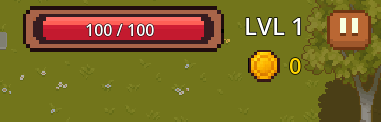
\includegraphics[width=0.9\linewidth]{image/hud.png}
		\caption{HUD - zdravotní lišta, level, zlato a pause tlačítko}
	\end{figure}
	
	\subsection{Zdravotní lišta}
	\nopagebreak
	
\begin{lstlisting}[style=GDScript, caption={Aktualizace zdravotní lišty}]
func _update_health_bar():
	if not player or not is_instance_valid(player):
		return
	
	var display_hp = player.current_hp
	if display_hp < 0:
		display_hp = 0
	
	# Výpočet procenta chybějícího zdraví
	var missing_health_percent = 1.0 - (float(display_hp) / float(player.max_hp))
	
	# Aktualizace šířky prázdné části
	var empty_width = max_bar_width * missing_health_percent
	health_bar_empty.size.x = empty_width
	health_bar_empty.position.x = -141.0 + (max_bar_width - empty_width)
	
	# Aktualizace textu
	health_text.text = str(display_hp) + " / " + str(player.max_hp)
\end{lstlisting}
	\newpage
	\subsection{Pause menu}
	\nopagebreak
	
	Pause menu zastavuje hru pomocí nastavení \texttt{Engine.time\_scale} na 0 a zobrazuje statistiky hráče:
	\nopagebreak
	
\begin{lstlisting}[style=GDScript, caption={Pause menu funkce}]
func show_pause_menu():
	visible = true
	Engine.time_scale = 0.0
	update_stats()

func hide_pause_menu():
	visible = false
	Engine.time_scale = 1.0

func _input(event):
	if event.is_action_pressed("ui_cancel"):  # ESC
		if visible:
			hide_pause_menu()
		else:
			show_pause_menu()
\end{lstlisting}

	\section{Main menu}
	\nopagebreak
	
	Hlavní menu obsahuje pozadí s loading screen obrázkem a custom tlačítka.

	\begin{figure}[h]
		\centering
		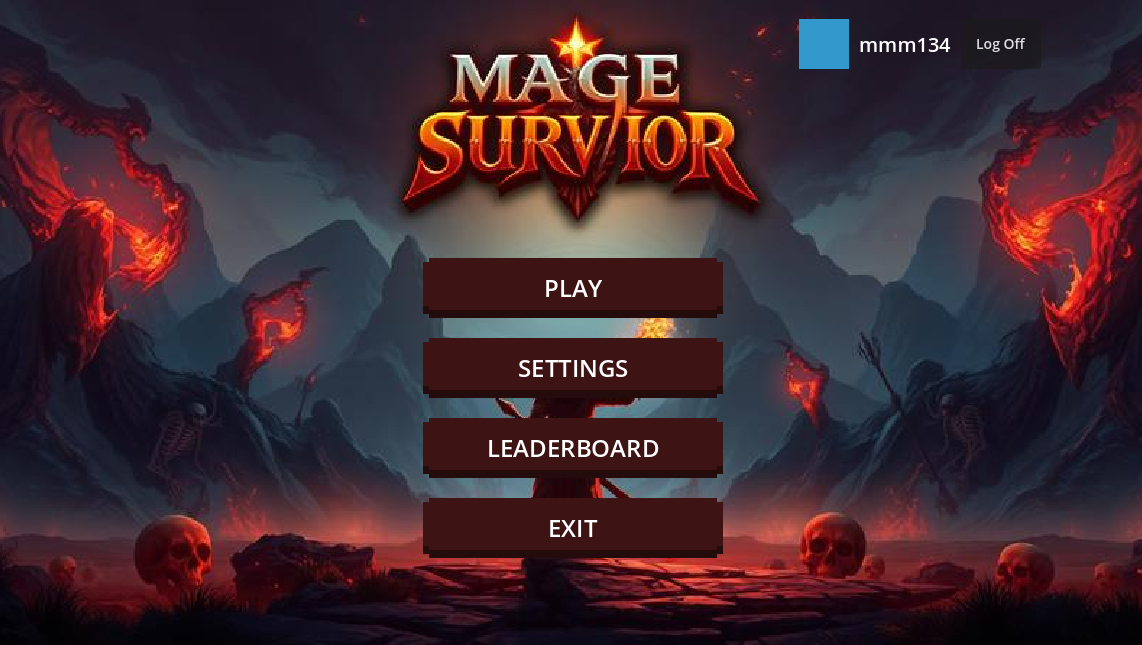
\includegraphics[width=0.8\linewidth]{image/main_menu.png}
		\caption{Hlavní menu hry}
	\end{figure}
	
	\subsection{TextureButton s labelem}
	\nopagebreak
	
	Pro estetická tlačítka byla použita kombinace TextureButton a Label. Každé tlačítko má přiřazenou texturu a Label potomek pro zobrazení textu, který je vystředěný pomocí anchor systému Godotu.

	\chapter*{Závěr}
	\addcontentsline{toc}{chapter}{Závěr}
	
	V rámci této závěrečné práce byl vytvořen kompletní funkční prototyp akční hry Mage Survivor v herním enginu Godot 4. Hra obsahuje všechny základní mechaniky žánru survivor -- vlny nepřátel, progresivní obtížnost, levelování a upgrade systém.
	
	Hlavními přínosy práce jsou:
	\begin{itemize}
		\item Implementace komplexního systému legendárních předmětů s pěti unikátními efekty
		\item Vytvoření ekonomického systému s progresivní cenou truhel
		\item Pokročilé vizuální efekty pomocí animovaných sprite částic
		\item Intuitivní uživatelské rozhraní s HUD a menu systémy
		\item Čistý a modulární kód v GDScriptu usnadňující budoucí rozšiřování
	\end{itemize}
	
	\section*{Možná budoucí vylepšení}
	
	Projekt má potenciál pro další rozšíření:
	\begin{itemize}
		\item Přidání dalších legendárních předmětů a jejich kombinací
		\item Implementace více typů nepřátel s různými schopnostmi
		\item Systém achievementů a statistik
		\item Různé mapy s unikátními prostředími
		\item Zvukové efekty a hudba
	\end{itemize}
	

	%% Seznam použitelných informačních zdrojů
	\renewcommand{\bibname}{Seznam použitelných informačních zdrojů}
	\nocite{*}
	
	\begin{thebibliography}{99}
		\bibitem{youtube1} \textit{Godot Tutorial Video} [online]. YouTube [cit. 2026-01-04]. Dostupné z: \url{https://www.youtube.com/watch?v=rckLxmH_fK0}
		
		\bibitem{godotPlayer} \textit{Your First 2D Game - Player Scene} [online]. Godot Engine Documentation [cit. 2026-01-04]. Dostupné z: \url{https://docs.godotengine.org/en/stable/getting_started/first_2d_game/02.player_scene.html}
		
		\bibitem{chatgpt} \textit{ChatGPT} [online]. OpenAI [cit. 2026-01-04]. Dostupné z: \url{https://chat.openai.com/}
		
		\bibitem{youtube2} \textit{Godot Tutorial Video} [online]. YouTube [cit. 2026-01-04]. Dostupné z: \url{https://www.youtube.com/watch?v=7ZAF_fn3VOc}
		
		\bibitem{youtube3} \textit{Godot Tutorial Video} [online]. YouTube [cit. 2026-01-04]. Dostupné z: \url{https://www.youtube.com/watch?v=GiZuWjXmvcc}
		
		\bibitem{reddit} \textit{r/godot - Godot Engine Community} [online]. Reddit [cit. 2026-01-04]. Dostupné z: \url{https://www.reddit.com/r/godot/}
		
		\bibitem{craftpix} \textit{CraftPix - Game Assets and Sprites} [online]. CraftPix [cit. 2026-01-04]. Dostupné z: \url{https://craftpix.net/categorys/sprites/}
		
		\bibitem{deepai} \textit{Text to Image AI Generator} [online]. DeepAI [cit. 2026-01-04]. Dostupné z: \url{https://deepai.org/machine-learning-model/text2im}
		
		\bibitem{googleai} \textit{Google AI Studio} [online]. Google [cit. 2026-01-04]. Dostupné z: \url{https://aistudio.google.com/apps}
		
		\bibitem{pixelart} \textit{Pixel Art Village} [online]. Pixel Art Village [cit. 2026-01-04]. Dostupné z: \url{https://pixelartvillage.com/}
	\end{thebibliography}

\end{document}
